\documentclass[10pt,x11names,table]{beamer}

\usetheme[progressbar=frametitle]{metropolis}
\usepackage{appendixnumberbeamer}
\usepackage{xcolor}

\usepackage{polyglossia}
\setmainlanguage{spanish}

\usepackage{listings}

\usepackage{booktabs}
\usepackage[scale=2]{ccicons}

\usepackage{pgfplots}
\usepgfplotslibrary{dateplot}

%ANIMACIONES
\usepackage{animate}
\usepackage{graphicx}
\usepackage[caption=false]{subfig}

\usepackage{xspace}

\newcommand*{\eg}{e.g.\@\xspace}
\newcommand*{\ie}{i.e.\@\xspace}

\let\oldquote\quote
\let\endoldquote\endquote
\renewenvironment{quote}[2][]
  {\if\relax\detokenize{#1}\relax
     \def\quoteauthor{#2}%
   \else
     \def\quoteauthor{#2~---~#1}%
   \fi
   \oldquote}
  {\par\nobreak\smallskip\hfill(\quoteauthor)%
   \endoldquote\addvspace{\bigskipamount}}
   
\usepackage{wrapfig}

\usepackage{subfig}
\usepackage{hyperref}
\usepackage{multicol}

\setbeamertemplate{bibliography item}[text]

\usepackage[font=small,skip=0pt, labelformat=empty]{caption}

\usepackage{dirtytalk}
\usepackage[acronym]{glossaries}
\makeglossaries

\newacronym{ae}{AE}{Autoencoder}
\newacronym{ai}{AI}{Artificial Intelligence}
\newacronym{brief}{BRIEF}{Binary Robust Independent Elementary Features}
\newacronym{cnn}{CNN}{Convolutional Neural Network}
\newacronym{diffit}{DiffiT}{Diffusion Vision Transformer}
\newacronym{dl}{DL}{Deep Learning}
\newacronym{fast}{FAST}{Features from Accelerated Segment Test}
\newacronym{gan}{GAN}{Generative Adversarial Network}
\newacronym{gpu}{GPU}{Graphics Processing Unit}
\newacronym{ilsvrc}{ILSVRC}{ImageNet Large Scale Visual Recognition Challenge}
\newacronym{nlp}{NLP}{Natural Language Processing}
\newacronym{nn}{NN}{Neural Network}
\newacronym{ocr}{OCR}{Optical Character Recognition}
\newacronym{sift}{SIFT}{Scale-Invariant Feature Transform}
\newacronym{slam}{SLAM}{Simultaneous Localization and Mapping}
\newacronym{surf}{SURF}{Speeded-Up Robust Features}
\newacronym{vae}{VAE}{Variational Autoencoder}
\newacronym{vgg}{VGG}{Visual Geometry Group}
\newacronym{vit}{ViT}{Vision Transformer}
\newacronym{yolo}{YOLO}{You Only Look Once}
\subtitle{Métodos Generativos, curso 2024-2025}

\date{\today}
\author{Guillermo Iglesias, guillermo.iglesias@upm.es \newline
Jorge Dueñas Lerín, jorge.duenas.lerin@upm.es  \newline
Félix Fuentes Hurtado, felix.fuentes@upm.es}

\institute{Escuela Técnica Superior de Ingeniería de Sistemas Informáticos | UPM \newline
\hbox{} \newline \ccbysa \hspace{0.1pt} \ccNonCommercial}

%%%%%%%%%%%%%%%%%%%%%%%%%%%%%%%%%%%%%       
\title{Vision Transformers (ViT)}

\begin{document}
\maketitle

\begin{frame}{Introducción}
Los \glspl{vit} son una arquitectura presentada en el artículo \textit{"An image is worth 16x16 words: Transformers for image recognition at scale"} del año 2020 \cite{dosovitskiy2020image} dentro del área de la \alert{visión por computador}.

\begin{itemize}
    \item Utilizan los mecanismos de \alert{atención} para procesar imágenes como \alert{secuencias de píxeles}
    \item Utilizan únicamente el \alert{encoder} para generar \alert{descriptores} de imágenes
\end{itemize}
\end{frame}

\begin{frame}{Características principales}
\begin{columns}[c]
\centering
\begin{column}{0.45\textwidth}
\alert{\Large Ventajas}
\begin{itemize}
    \item Captura \alert{dependencias globales} de la imagen, es decir, correlaciona elementos muy distantes
    \item Mejora los resultados a la hora de intepretar o generar imágenes
    \item Simplifican el \alert{condicionamiento} de las arquitecturas
\end{itemize}
\end{column}
\centering
\begin{column}{0.45\textwidth}
\alert{\Large Desventajas}
\begin{itemize}
    \item Necesidad de \alert{grandes datasets}
    \begin{itemize}
        \item Muchas veces se contrarresta con un \alert{pretraining}, pero no siempre es posible, y sigue siendo muy costoso
        \item Hay investigación que intenta reducir el coste \cite{yuan2021tokens}
    \end{itemize}
\end{itemize}
\end{column}
\end{columns}
\end{frame}

\begin{frame}{Metodología de los ViT}
Los principales pasos en un \gls{vit} son los siguientes:
\begin{enumerate}
    \item Tokenización de la imagen
    \item Procesamiento de tokens
    \item Encoding de los tokens
    \item Procesamiento con \gls{nn}
    \item Generación de la salida
\end{enumerate}
\end{frame}

\begin{frame}{Tokenización de la imagen}
De la misma manera que los Transformers en \alert{\gls{nlp}} necesitan que el texto sea procesado para ser entendible por un modelo de \gls{ai}, las imágenes han de ser \alert{preprocesadas} para ser tratadas.

\begin{figure}
    \centering
    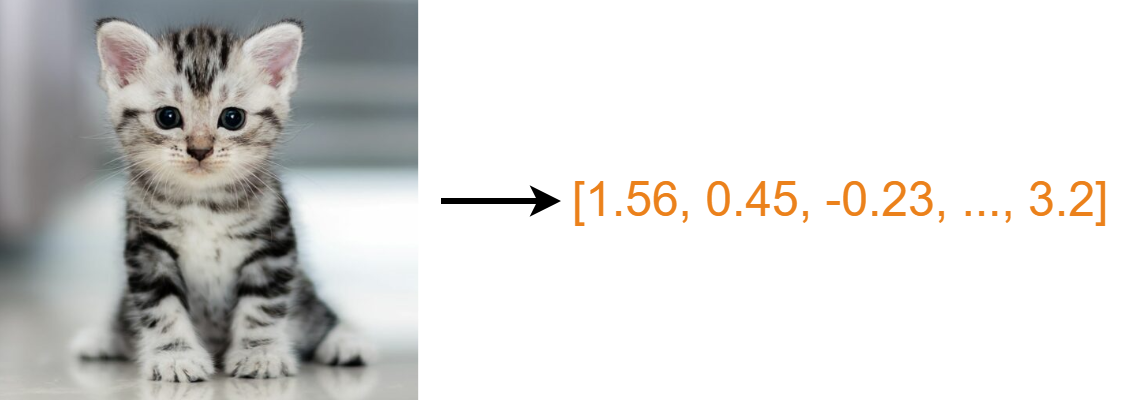
\includegraphics[width=0.8\textwidth]{figures/Vision_Transformers/Image_Preprocessing.png}
\end{figure}
\end{frame}

\begin{frame}{Tokenización de la imagen: Generación de parches}
Los \gls{vit} procesan una imagen como una \alert{secuencia de tokens}. Cada token es un \alert{parche} de la imagen total, de tamaño $P_HxP_WxC$ (alto, ancho, canales).

\begin{figure}
    \centering
    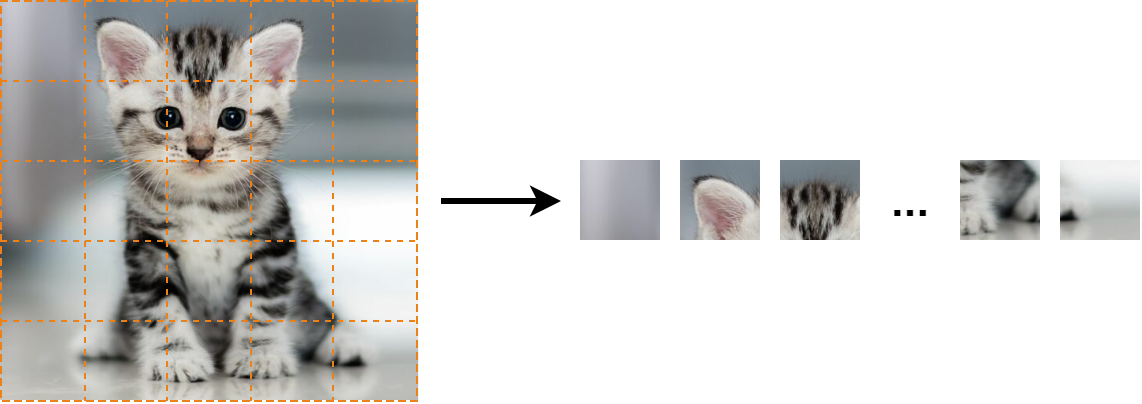
\includegraphics[width=0.8\textwidth]{figures/Vision_Transformers/Image_Tiling.png}
\end{figure}

*El tamaño más estándar para los parches es 16x16 píxeles
\end{frame}

\begin{frame}{Tokenización de la imagen: Flatten de parches}
Cada parche es \alert{vectorizado} aplicando un flatten.

\begin{figure}
    \centering
    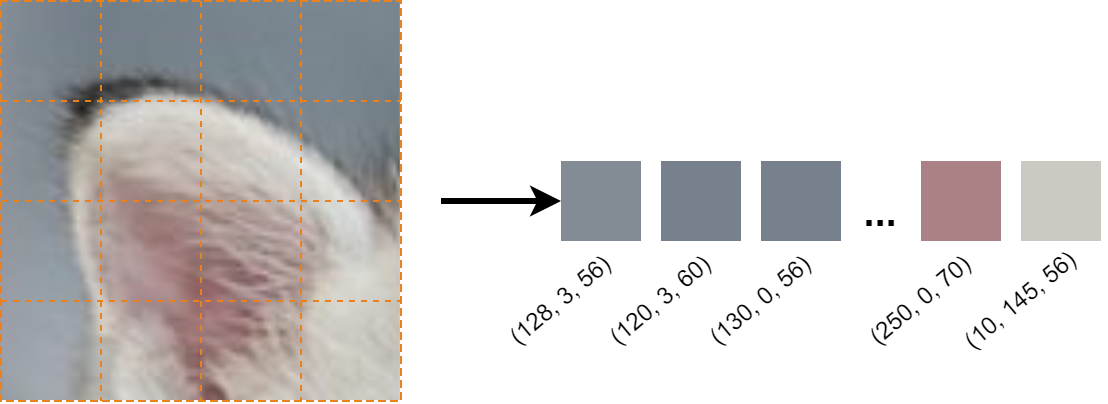
\includegraphics[width=0.8\textwidth]{figures/Vision_Transformers/Patch_Flatten.png}
\end{figure}

Cada posición representa el valor de color del píxel.
\end{frame}

\begin{frame}{Tokenización de la imagen: Proyección linear de los tokens}
Una práctica común es proyectar los tokens a un espacio latente de un tamaño arbitrario. Se utiliza para mejorar la \alert{representación de los parches}, lo que es equivalente a los \alert{embeddings de palabras} en \gls{nlp}. 

\begin{figure}
    \centering
    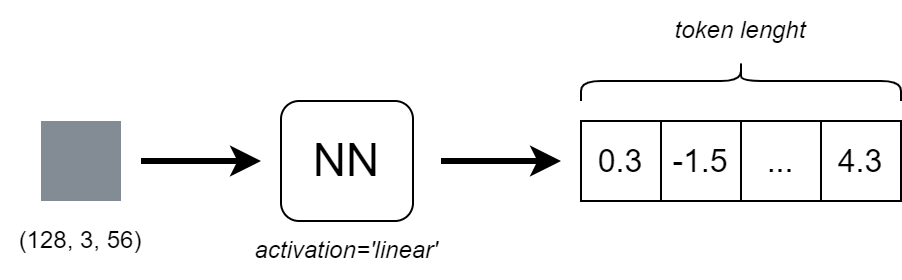
\includegraphics[width=0.8\textwidth]{figures/Vision_Transformers/Token_Projection.png}
\end{figure}

*En \cite{dosovitskiy2020image} el \textit{token lenght} se define a 768.
\end{frame}

\begin{frame}{Tokenización de la imagen: Resumen}
Con todo el proceso definido anteriormente, es posible generar una \alert{representación latente} de una imagen, dividida en parches, que además pueden adaptarse al proceso de \alert{aprendizaje}. 

\begin{figure}
    \centering
    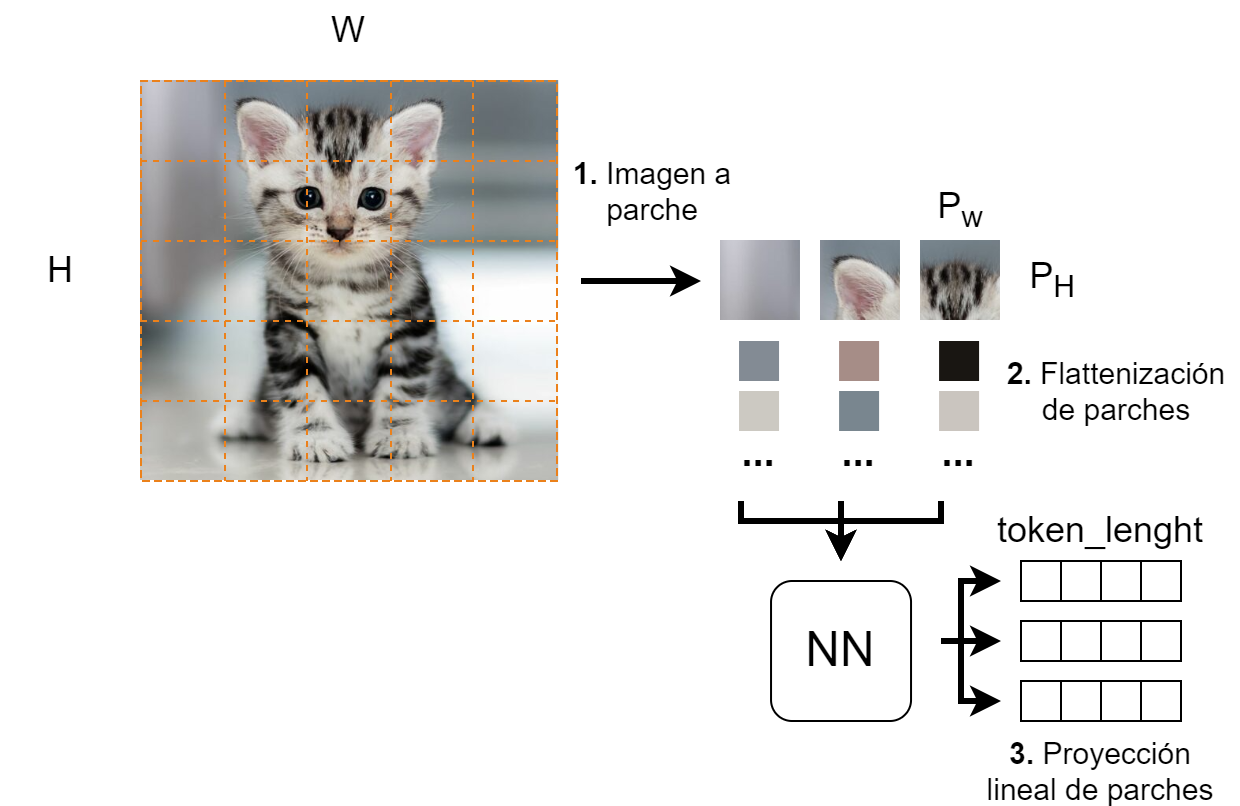
\includegraphics[width=0.8\textwidth]{figures/Vision_Transformers/Image_Tokenization_Process.png}
\end{figure}
\end{frame}

\begin{frame}{Procesamiento de tokens}
El siguiente paso consiste en procesar los tokens para añadir \alert{información extra} necesaria para mantener las relaciones espaciales y generar una salida.

\begin{figure}
    \centering
    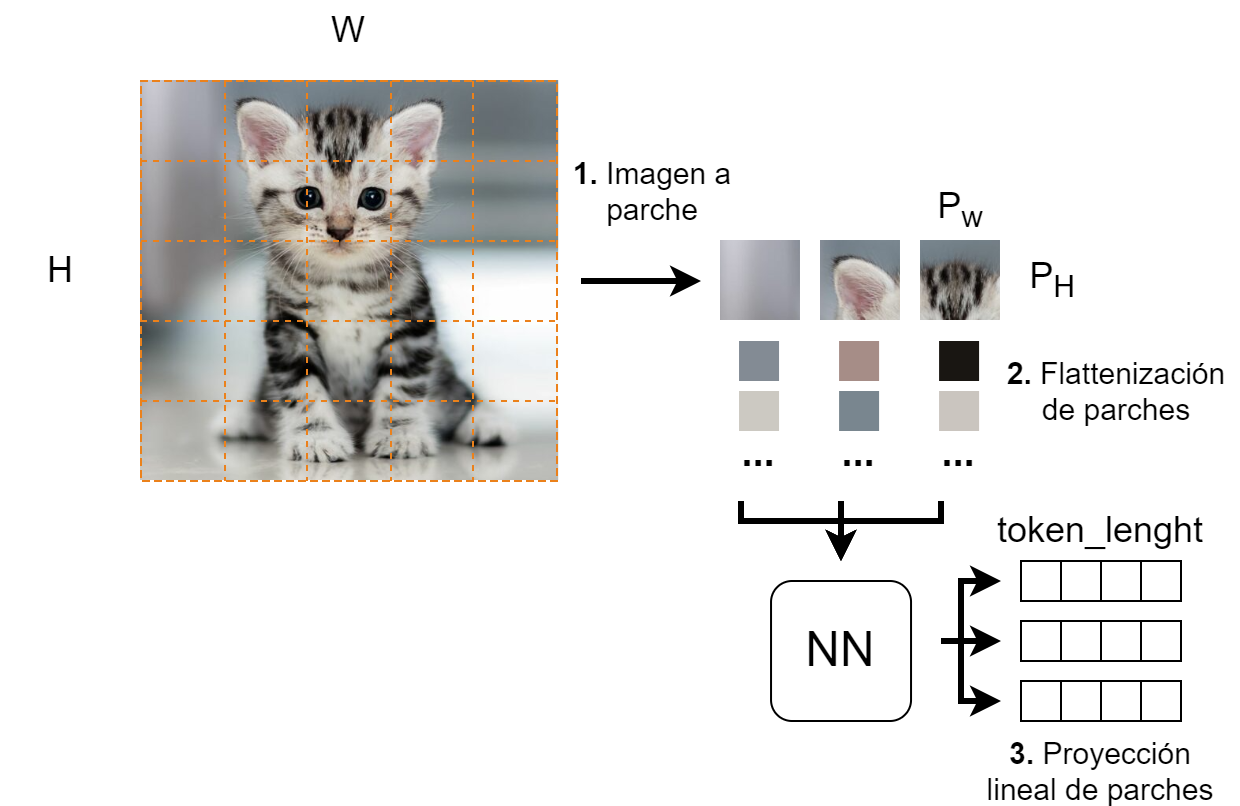
\includegraphics[width=0.8\textwidth]{figures/Vision_Transformers/Image_Tokenization_Process.png}
\end{figure}
\end{frame}

\begin{frame}{Procesamiento de tokens: Concatenar el \textit{prediction token}}
El \alert{\textit{prediction token}} es un vector que siempre se inicializa a \alert{0}, usado para generar la salida de \alert{predicción tras en encoding}.

\begin{figure}
    \centering
    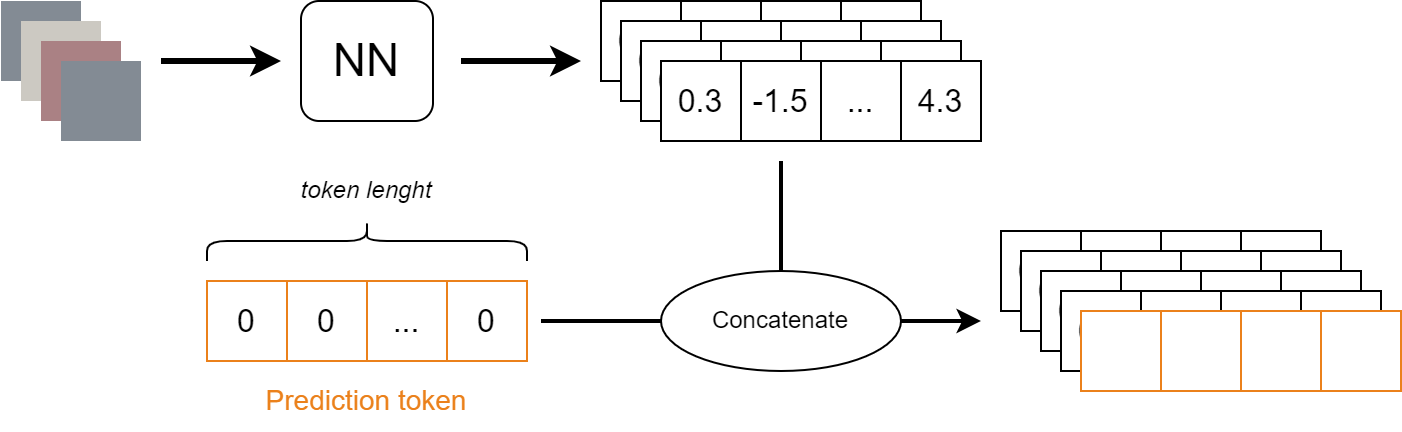
\includegraphics[width=\textwidth]{figures/Vision_Transformers/Pred_Token.png}
\end{figure}
\end{frame}

\begin{frame}{Procesamiento de tokens: Position embedding}
Para mantener las \alert{relaciones espaciales} de los parches de una imagen se añade un \alert{positional embedding} que \alert{ordena} los embeddings. Esto ya se hacía en los \alert{Transformers} para \gls{nlp}.

\begin{figure}
    \centering
    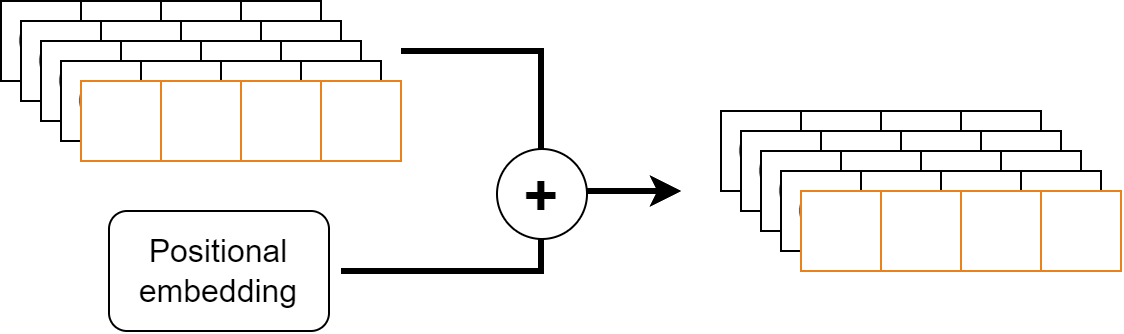
\includegraphics[width=0.8\textwidth]{figures/Vision_Transformers/Pos_Embedding.png}
\end{figure}

*Es importante recalcar que el positional embedding es \alert{sumado} a los anteriores. Normalmente se una una función \alert{sinusoidal}.
\end{frame}

\begin{frame}{Encoding}
La información generada previamente se procesa con \alert{bloques de encoding} usando capas de \alert{atención}. Se sigue el mismo procedimiento que en los \alert{Transformers vanilla}. 

\begin{figure}
    \centering
    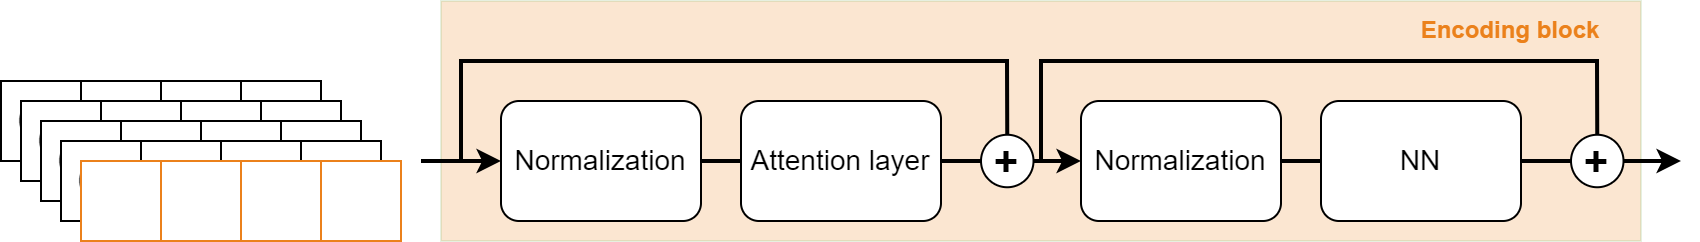
\includegraphics[width=\textwidth]{figures/Vision_Transformers/Encoding_Block.png}
\end{figure}
\end{frame}

\begin{frame}{Encoding: Intuición}
En este punto cabe recordar que el \alert{encoder} está procesando cada parche de la imagen, \alert{proyectado} a un espacio latente que guarda las \alert{relaciones entre parches}. De esta forma es posible \alert{extraer características} de las imágenes.

\begin{figure}
    \centering
    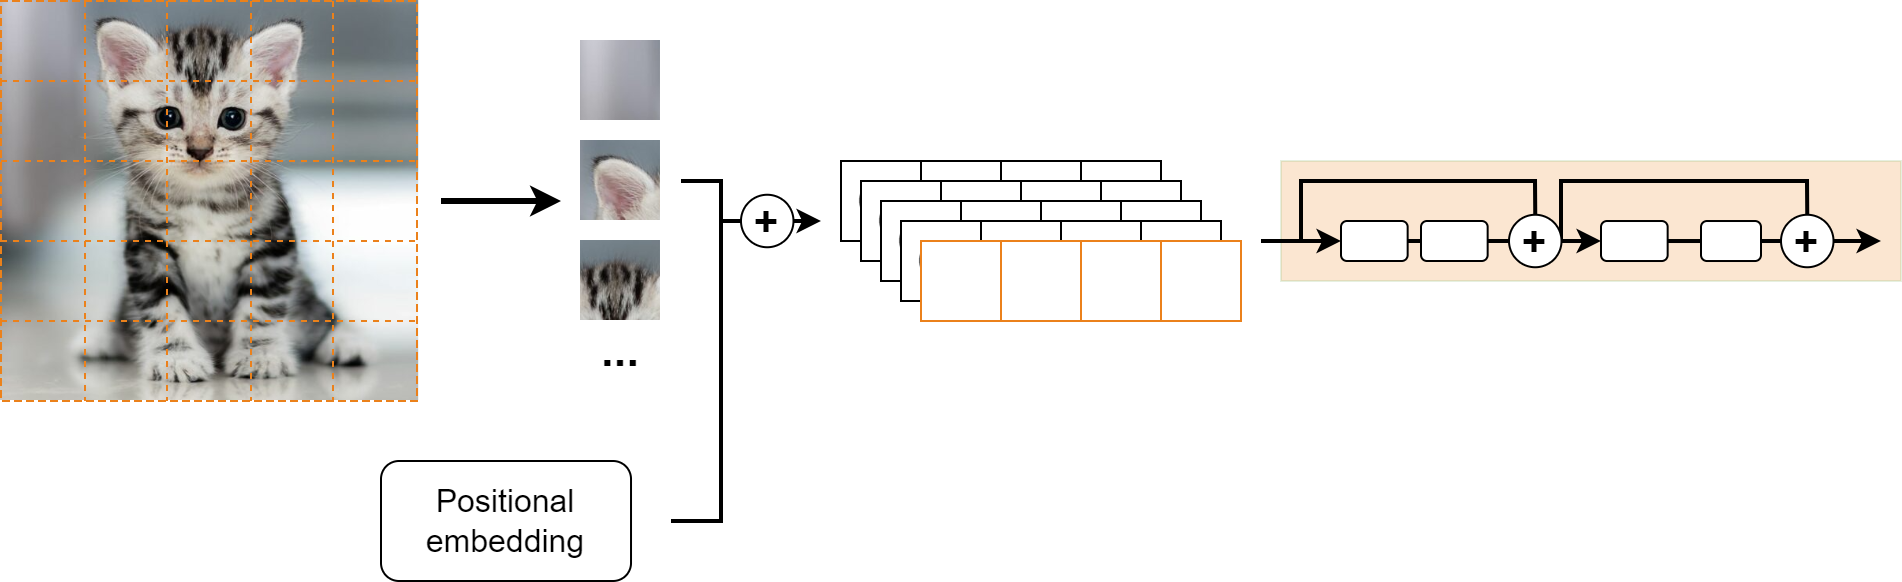
\includegraphics[width=\textwidth]{figures/Vision_Transformers/Encoding_Processing.png}
\end{figure}
\end{frame}

\begin{frame}{Salida del modelo}
Una vez procesada la información, se genera la \alert{salida} de la red de neuronas. Hasta este punto, la arquitectura del \gls{vit} es general y puede usarse para múltiples problemas. Pero en este ejemplo se explicará cómo hacer una \alert{clasificación}.

Para ello se usa el \alert{prediction token} anteriormente definido.

\begin{figure}
    \centering
    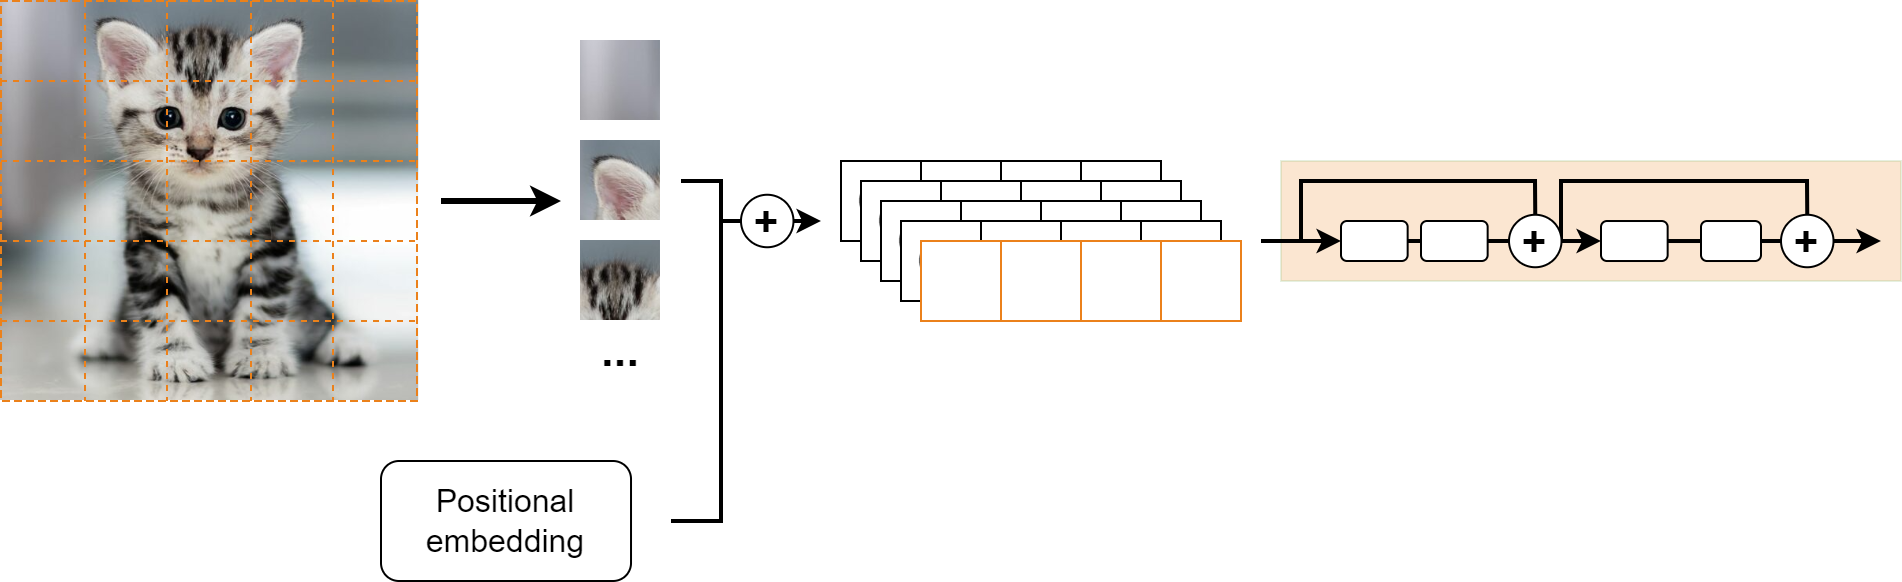
\includegraphics[width=\textwidth]{figures/Vision_Transformers/Encoding_Processing.png}
\end{figure}
\end{frame}

\begin{frame}{Salida del modelo}
El prediction token es finalmente procesado por una \alert{cabeza de clasificación} compuesta por un \alert{perceptrón}.

Normalmente, este perceptrón no es más que una capa con activación lineal.

\begin{figure}
    \centering
    
\includegraphics[width=0.8\textwidth]{figures/Vision_Transformers/Output.png}
\end{figure}
\end{frame}

\begin{frame}{Generación de contenido: DiffiT}
Existen arquitecturas como \alert{\gls{diffit}} \cite{hatamizadeh2024diffit} que combinan la potencia de los \gls{vit} con la capacidad de generación de los \alert{Diffusion models} para generar contenido.

\begin{figure}
    \centering
    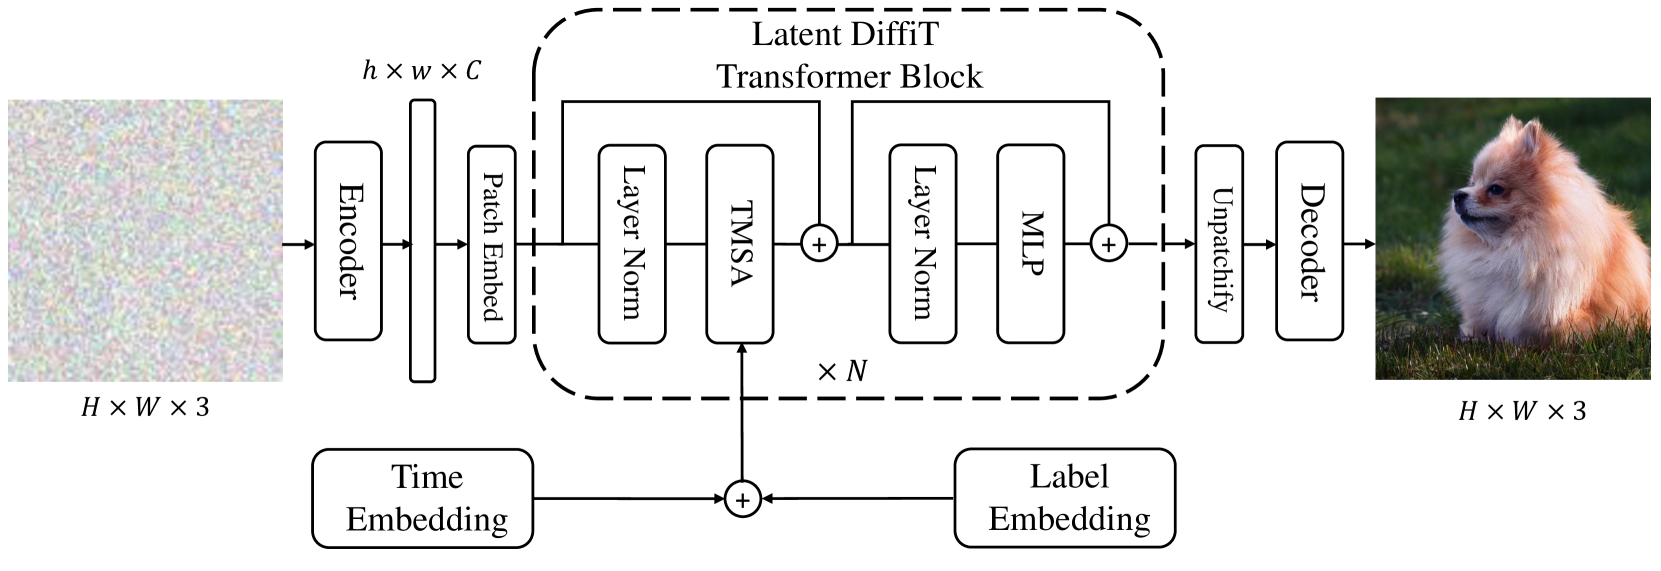
\includegraphics[width=\textwidth]{figures/Vision_Transformers/DiffiT_Architecture.png}
    \caption{\cite{hatamizadeh2024diffit}}
\end{figure}
\end{frame}

\begin{frame}{Generación de contenido: DiffiT}
Combinando una arquitectura de \alert{\gls{ae}} e introduciendo bloques de \gls{vit} con un \alert{embedding temporal} consiguen generar los mejores resultados del estado del arte.

\begin{figure}
    \centering
    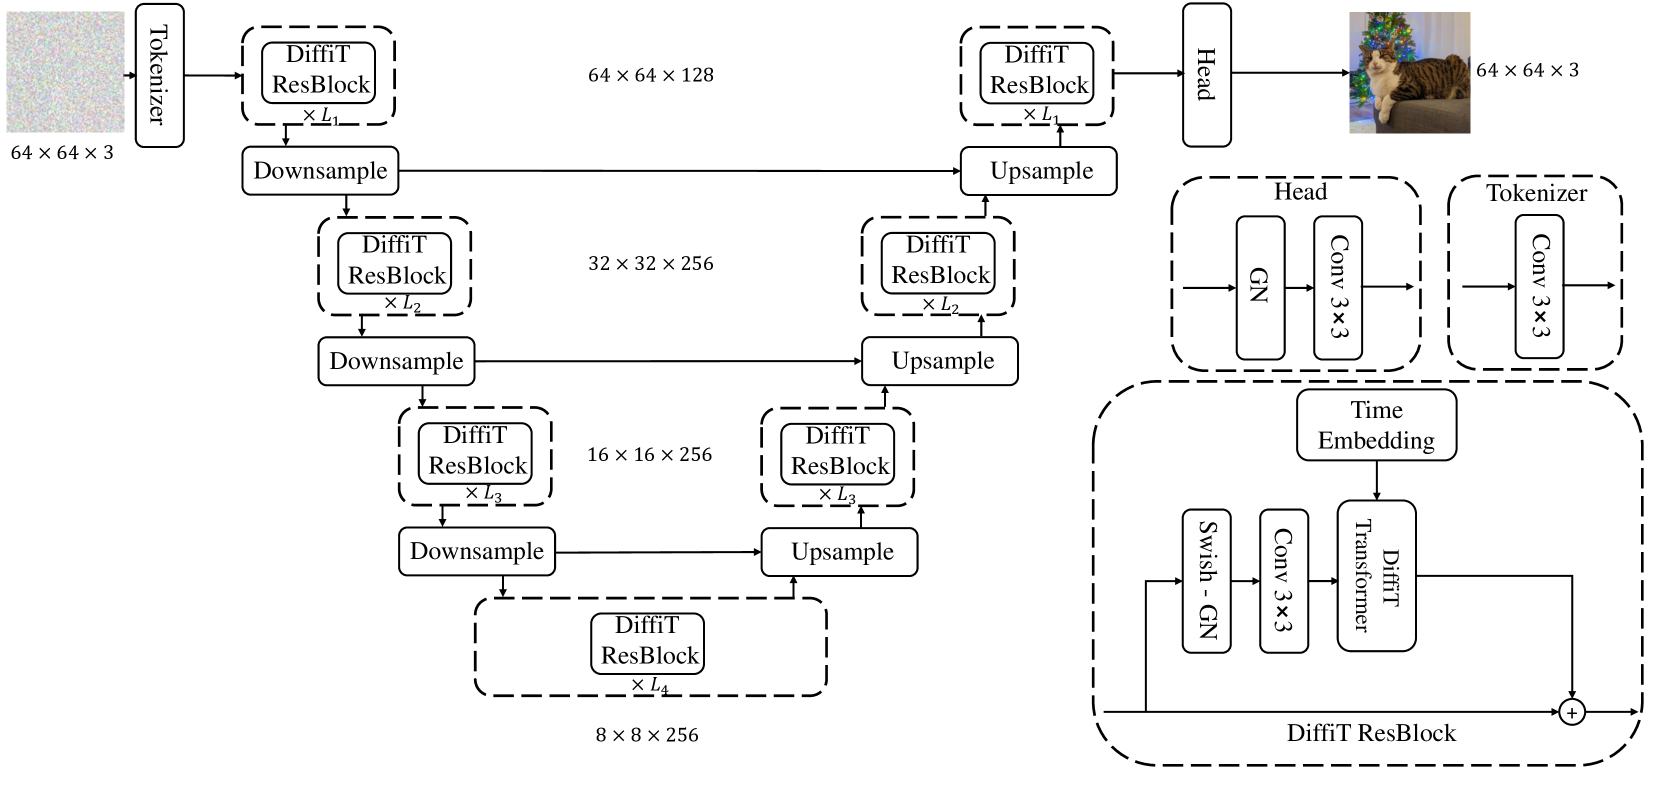
\includegraphics[width=\textwidth]{figures/Vision_Transformers/DiffiT_Transformer.png}
    \caption{\cite{hatamizadeh2024diffit}}
\end{figure}
\end{frame}

\addcontentsline{toc}{section}{Referencias}

\begin{frame}[allowframebreaks]{Referencias}
    \bibliographystyle{unsrt}
    \bibliography{references.bib}
\end{frame}

\end{document}